\renewcommand*{\arraystretch}{1.1}

\subsection*{BI / read / 14}
\label{section:bi-read-14}

\noindent\begin{tabularx}{\queryCardWidth}{|>{\queryPropertyCell}p{\queryPropertyCellWidth}|X|}
	\hline
	query & BI / read / 14 \\ \hline
%
	title & Top thread initiators
 \\ \hline
%
	pattern & \hfill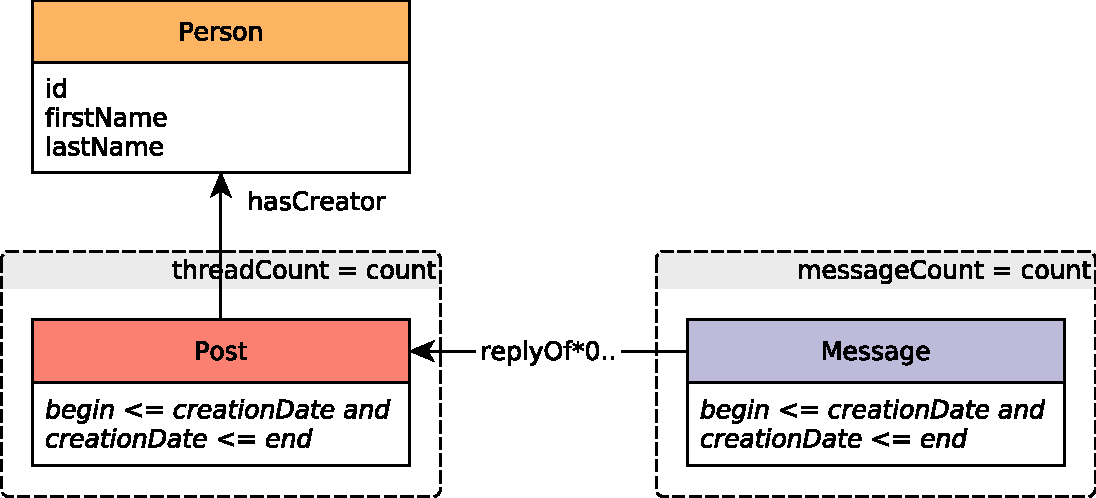
\includegraphics[scale=\patternscale,margin=0cm .2cm]{patterns/bi-read-14}\hfill\vadjust{} \\ \hline
%
	desc. & For each \emph{Person}, count the number of \emph{Posts} they created in
the time interval \texttt{{[}startDate,\ endDate{]}} (equivalent to the
number of threads they initiated) and the number of \emph{Messages} in
each of their (transitive) reply trees. When calculating \emph{Message}
counts only consider messages created within the given time interval.

Return each \emph{Person}, number of \emph{Posts} they created, and the
count of all \emph{Messages} that appeared in the reply trees (including
\emph{Post} at tree root) they created.
 \\ \hline
%
	
		params &
		\innerCardVSpace{\begin{tabularx}{\attributeCardWidth}{|>{\paramNumberCell}c|>{\varNameCell}M|>{\typeCell}m{\typeWidth}|Y|} \hline
		$\mathsf{1}$ & startDate
 & Date
 &  \\ \hline
		$\mathsf{2}$ & endDate
 & Date
 &  \\ \hline
		\end{tabularx}}\innerCardVSpace \\ \hline
	
%
	
		result &
		\innerCardVSpace{\begin{tabularx}{\attributeCardWidth}{|>{\resultNumberCell}c|>{\varNameCell}M|>{\typeCell}m{\typeWidth}|>{\resultOriginCell}c|Y|} \hline
		$\mathsf{1}$ & person.id & 64-bit Integer & R &
				 \\ \hline
		$\mathsf{2}$ & person.firstName & String & R &
				 \\ \hline
		$\mathsf{3}$ & person.lastName & String & R &
				 \\ \hline
		$\mathsf{4}$ & postCount & 32-bit Integer & A &
				The number of \emph{Posts} created by that \emph{Person} (the number of
threads initiated)
 \\ \hline
		$\mathsf{5}$ & messageCount & 32-bit Integer & A &
				The number of \emph{Messages} created in all the threads this
\emph{Person} initiated
 \\ \hline
		\end{tabularx}}\innerCardVSpace \\ \hline
	
%
	
		sort		&
		\innerCardVSpace{\begin{tabularx}{\attributeCardWidth}{|>{\sortNumberCell}c|>{\varNameCell}M|>{\directionCell}c|Y|} \hline
		$\mathsf{1}$ & messageCount
 & $\desc
$ &  \\ \hline
		$\mathsf{2}$ & person.id
 & $\asc
$ &  \\ \hline
		\end{tabularx}}\innerCardVSpace \\ \hline
	%
	limit & 100 \\ \hline
	%
	CPs &
	\multicolumn{1}{>{\raggedright}l|}{
		\chokePoint{1.2}, 
		\chokePoint{2.2}, 
		\chokePoint{2.3}, 
		\chokePoint{3.2}, 
		\chokePoint{7.2}, 
		\chokePoint{7.3}, 
		\chokePoint{7.4}
		} \\ \hline
	%
	%
\end{tabularx}
\queryCardVSpace